\documentclass[12pt, a4paper]{article}

%% ── Packages ──────────────────────────────────────────────────────────────────
\usepackage[T1]{fontenc}
\usepackage[utf8]{inputenc}
\usepackage[english]{babel}
\usepackage{geometry}
\geometry{margin=2.5cm}

\usepackage{booktabs}       % \toprule \midrule \cmidrule \bottomrule
\usepackage{xcolor}         % \definecolor \cellcolor \rowcolor
\usepackage{colortbl}       % needed by xcolor for table cells
\usepackage{multirow}       % \multirow
\usepackage{siunitx}        % S column type (decimal-aligned)
\usepackage{array}          % extended column spec
\usepackage{caption}        % better caption formatting
\usepackage{amsmath}        % \mathrm
\usepackage{microtype}      % better justification
\usepackage{graphicx}       % \includegraphics
\usepackage{subcaption}     % subfigure captions

%% ── Colors ────────────────────────────────────────────────────────────────────
\definecolor{hdrblue}{RGB}{30, 64, 110}
\definecolor{hdrlight}{RGB}{220, 232, 248}
\definecolor{rowalt}{RGB}{245, 248, 252}

%% ── Helpers ───────────────────────────────────────────────────────────────────
\newcommand{\hcell}[1]{\cellcolor{hdrblue}\textcolor{white}{\textbf{#1}}}
\newcommand{\shcell}[1]{\cellcolor{hdrlight}\textbf{#1}}

%% ── siunitx setup ─────────────────────────────────────────────────────────────
\sisetup{
  detect-weight = true,
  detect-inline-weight = math,
}

%% ── Caption style ─────────────────────────────────────────────────────────────
\captionsetup{
  font      = small,
  labelfont = bf,
  skip      = 6pt,
}

%% ──────────────────────────────────────────────────────────────────────────────
\begin{document}

\begin{table}[h]
\centering
\caption{%
  Geometry of triangle $Q$\,--\,$C$\,--\,GT across 196 queries.
  $C$ denotes the L2-normalised centroid of all G3 documents (oracle, LLM
  score\,=\,1.0) for each query.
  Spherical angles are derived from angular side lengths on the unit
  hypersphere; flat angles are derived from Euclidean (chord) side lengths.
  Note that Cosine and Angular distance are monotone transforms of each other
  and therefore yield identical vertex angles.
}
\label{tab:triangle_geometry}

%% ── Part 1 : Sides ────────────────────────────────────────────────────────────
\renewcommand{\arraystretch}{1.3}
\begin{tabular}{%
  >{\bfseries}l                           % side label (bold)
  S[table-format=1.2]                     % cosine Mean
  S[table-format=1.2]                     % cosine Med
  S[table-format=1.2]                     % cosine Min
  S[table-format=1.2]                     % cosine Max
  S[table-format=1.2]                     % euclidean Mean
  S[table-format=1.2]                     % euclidean Med
  S[table-format=1.2]                     % euclidean Min
  S[table-format=1.2]                     % euclidean Max
}
\toprule
\multirow{1}{*}{\hcell{\quad Side}}
  & \multicolumn{4}{c}{\shcell{Cosine distance}}
  & \multicolumn{4}{c}{\shcell{Euclidean distance}} \\
\cmidrule(lr){2-5}
\cmidrule(lr){6-9}
  & {\small\textit{Mean}}
  & {\small\textit{Med}}
  & {\small\textit{Min}}
  & {\small\textit{Max}}
  & {\small\textit{Mean}}
  & {\small\textit{Med}}
  & {\small\textit{Min}}
  & {\small\textit{Max}} \\
\midrule
$Q \!\to\! \mathrm{GT}$
  & 0.17 & 0.15 & 0.06 & 0.65
  & 0.58  & 0.56  & 0.35  & 1.14 \\
\rowcolor{rowalt}
$Q \!\to\! C$
  & 0.17 & 0.15 & 0.07 & 0.48
  & 0.57  & 0.55  & 0.38  & 0.98 \\
$C \!\to\! \mathrm{GT}$
  & 0.10 & 0.09 & 0.02 & 0.47
  & 0.43  & 0.41  & 0.22  & 0.97 \\
\bottomrule
\end{tabular}

\vspace{1.2em}

%% ── Part 2 : Angles ───────────────────────────────────────────────────────────
\begin{tabular}{%
  >{\bfseries}l
  S[table-format=3.1]
  S[table-format=3.1]
  S[table-format=3.1]
  S[table-format=3.1]
  S[table-format=3.1]
  S[table-format=3.1]
  S[table-format=3.1]
  S[table-format=3.1]
}
\toprule
\multirow{1}{*}{\hcell{\quad Vertex angle}}
  & \multicolumn{4}{c}{\shcell{Cosine (Spherical, \si{\degree})}}
  & \multicolumn{4}{c}{\shcell{Flat --- Euclidean (\si{\degree})}} \\
\cmidrule(lr){2-5}
\cmidrule(lr){6-9}
  & {\small\textit{Mean}}
  & {\small\textit{Med}}
  & {\small\textit{Min}}
  & {\small\textit{Max}}
  & {\small\textit{Mean}}
  & {\small\textit{Med}}
  & {\small\textit{Min}}
  & {\small\textit{Max}} \\
\midrule
$\angle Q$\;(apex)
  & 45.7 & 45.5 & 24.9 &  73.1
  & 43.6 & 43.8 & 21.7 &  69.4 \\
\rowcolor{rowalt}
$\angle C$\;(centroid)
  & 70.8 & 70.6 & 41.8 & 100.5
  & 68.2 & 68.0 & 37.6 &  96.3 \\
$\angle \mathrm{GT}$
  & 70.6 & 69.7 & 48.8 &  95.7
  & 68.1 & 67.7 & 46.8 &  93.5 \\
\cmidrule(lr){2-5}
\cmidrule(lr){6-9}
\rowcolor{rowalt}
Sum
  & \bfseries 187.0
  & \bfseries 186.3
  & \bfseries 183.1
  & \bfseries 213.4
  & \bfseries 180.0
  & \bfseries 180.0
  & \bfseries 180.0
  & \bfseries 180.0 \\
\bottomrule
\end{tabular}

\end{table}

%% ── Heatmap figure ────────────────────────────────────────────────────────────
\begin{figure}[h]
\centering
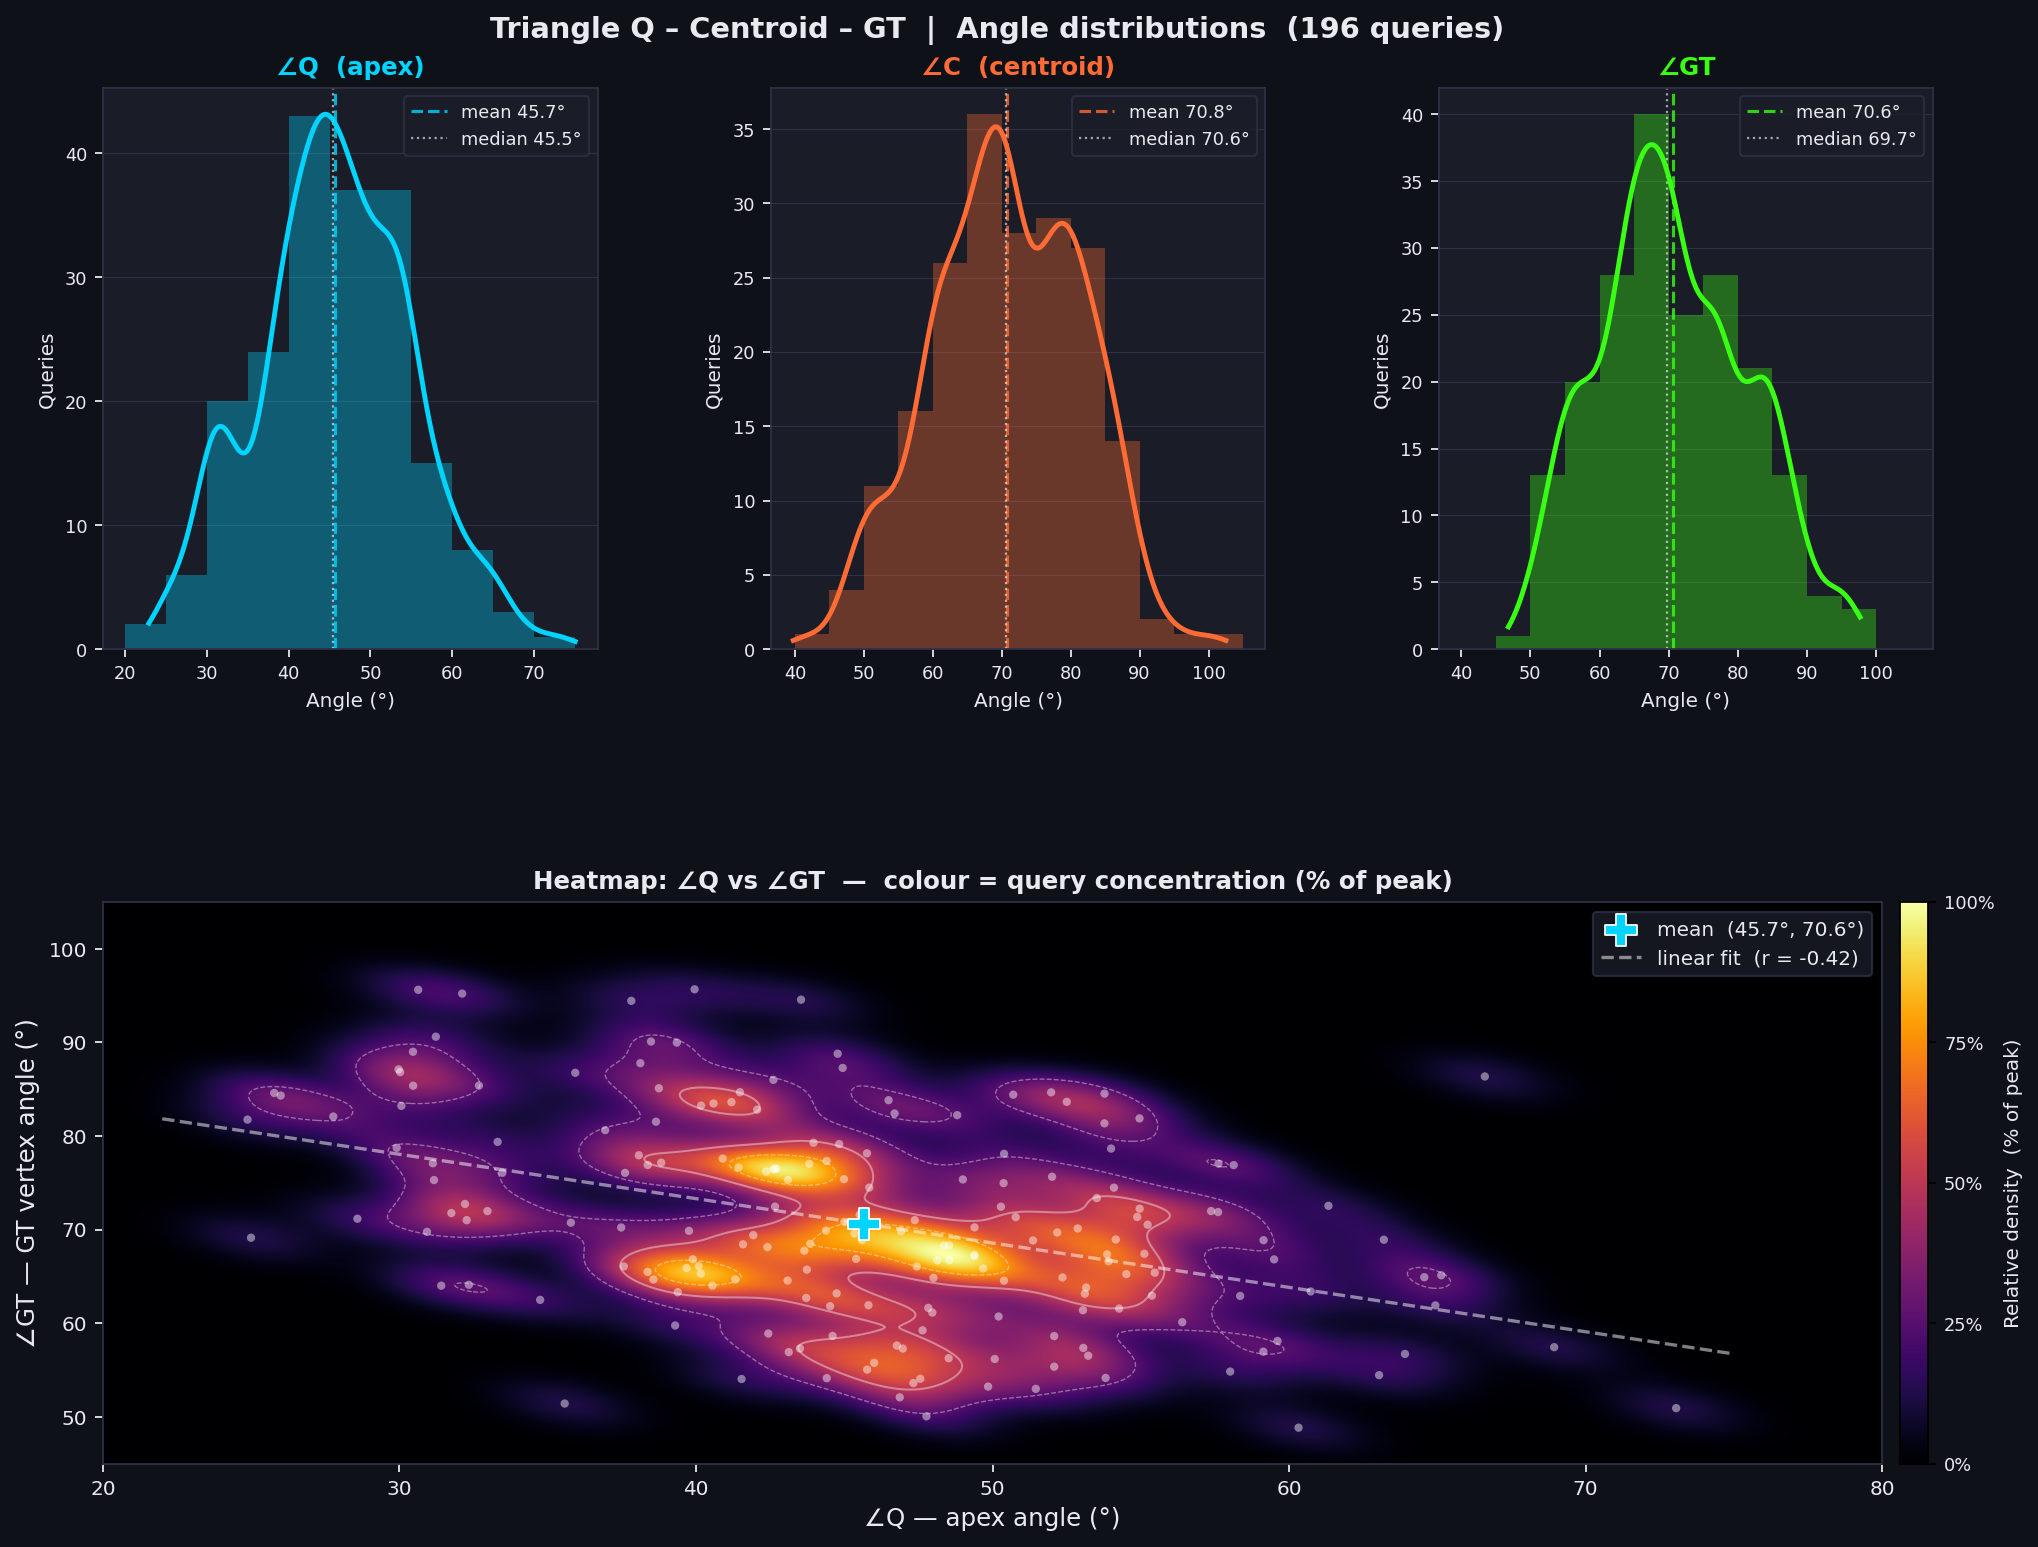
\includegraphics[width=0.88\textwidth]{triangle_heatmap.png}
\caption{%
  Heatmap of GT positions with Q fixed at the origin and C (G3 centroid) fixed
  along the x-axis at mean cosine distance 0.17.
  Each point is the 2D projection of GT for one query, computed from the three
  cosine side lengths via the law of cosines.
  Point colour encodes $\angle\mathrm{GT}$ (the vertex angle at the
  ground-truth document); the density contours show the joint distribution of
  GT positions across all 196 queries.
  The cluster tightly occupies the region above the Q--C axis, confirming that
  GT is consistently off-axis relative to the centroid direction.
}
\label{fig:gt_heatmap}
\end{figure}

%% ── Distribution tables ───────────────────────────────────────────────────────
\begin{table}[h]
\centering
\caption{Angle distributions (bin width 10\si{\degree}, $N=196$ queries)}
\label{tab:angle_hist}
\renewcommand{\arraystretch}{1.2}
\begin{tabular}{lrrr|lrrr}
\toprule
\multicolumn{4}{c|}{\textbf{$\angle Q$ (apex) --- Cosine/Spherical}}
  & \multicolumn{4}{c}{\textbf{$\angle\mathrm{GT}$ --- Cosine/Spherical}} \\
\textit{Range} & $n$ & \% & & \textit{Range} & $n$ & \% & \\
\midrule
{[}20--30)\si{\degree} &  8 &  4.1 & &  {[}50--60)\si{\degree} & 33 & 16.8 & \\
{[}30--40)\si{\degree} & 44 & 22.4 & &  {[}60--70)\si{\degree} & 68 & 34.7 & \\
\rowcolor{hdrlight}
\bfseries{[}40--50)\si{\degree} & \bfseries 80 & \bfseries 40.8 & & \bfseries{[}70--80)\si{\degree} & \bfseries 53 & \bfseries 27.0 & \\
{[}50--60)\si{\degree} & 52 & 26.5 & &  {[}80--90)\si{\degree} & 34 & 17.3 & \\
{[}60--70)\si{\degree} & 11 &  5.6 & &  {[}90--100)\si{\degree} &  7 &  3.6 & \\
\bottomrule
\end{tabular}
\end{table}

%% ── Conditional: ∠C given ∠GT ────────────────────────────────────────────────
\begin{table}[h]
\centering
\caption{%
  $\angle C$ (centroid vertex angle) conditional on $\angle\mathrm{GT}$ bin.
  Pearson correlation: $r(\angle\mathrm{GT},\,\angle C) = -0.668$.
  When $\angle\mathrm{GT}$ is sharp, the centroid deflects further from the GT
  direction (larger $\angle C$), a direct consequence of the fixed angle sum
  ($\approx187\si{\degree}$).
}
\label{tab:conditional_angles}
\renewcommand{\arraystretch}{1.25}
\begin{tabular}{lrrrr}
\toprule
$\angle\mathrm{GT}$ bin & $n$
  & $\angle C$ mean & $\angle C$ std & $\angle Q$ mean \\
\midrule
{[}50--60)\si{\degree} & 33 & 81.5\si{\degree} & 8.0\si{\degree} & 50.5\si{\degree} \\
\rowcolor{rowalt}
{[}60--70)\si{\degree} & 68 & 74.4\si{\degree} & 7.5\si{\degree} & 47.6\si{\degree} \\
{[}70--80)\si{\degree} & 53 & 67.1\si{\degree} & 8.5\si{\degree} & 44.5\si{\degree} \\
\rowcolor{rowalt}
{[}80--90)\si{\degree} & 34 & 61.5\si{\degree} & 10.0\si{\degree} & 40.6\si{\degree} \\
{[}90--100)\si{\degree} &  7 & 56.6\si{\degree} &  6.3\si{\degree} & 36.3\si{\degree} \\
\midrule
\multicolumn{2}{l}{\textit{All queries (196)}}
  & 70.8\si{\degree} & 9.3\si{\degree} & 45.7\si{\degree} \\
\bottomrule
\end{tabular}
\end{table}

\end{document}
